\documentclass[conference]{IEEEtran}

% ---------- PACKAGES ----------
\usepackage[utf8]{inputenc}
\usepackage{graphicx}
\usepackage{amsmath, amssymb}
\usepackage{booktabs}
\usepackage{multirow}
\usepackage{tabularx}
\usepackage{float}
\usepackage{caption}
\usepackage{subcaption}
\usepackage{lipsum}
\usepackage{url}
\usepackage{cite}
\usepackage{url}


% ---------- TABLE ADJUSTMENT ----------
\usepackage{adjustbox}
\usepackage{longtable}  % Nếu cần bảng nhiều dòng
\usepackage{stfloats}   % Cho phép table* nằm dưới cuối trang

% ---------- BEGIN DOCUMENT ----------
\begin{document}

% ---------- TITLE ----------
\title{Overcoming Data Imbalance and Feature Bias in Autism Classification with Overall Local Accuracy}

\author{
Thanh Nguyen Van Quoc $^{1}$, Hao Nguyen Thi Bich $^{2}$, Nhut Nguyen Minh$^{3}$, Thuan Nguyen Dinh$^{4}$\\
\textit{Faculty of Information Systems} \\
\textit{University of Information Technology - Vietnam National University} \\
Ho Chi Minh City, Vietnam \\
\{21521447@gm.uit.edu.vn, 21522049@gm.uit.edu.vn, nhutnm.17@grad.uit.edu.vn, thuannd@uit.edu.vn\}
}

% \author{
%     \IEEEauthorblockN{Author One, Author Two}
%     \IEEEauthorblockA{
%         Department, University \\
%         Email: \{author1, author2\}@univ.edu}
% }

\maketitle
\IEEEpeerreviewmaketitle

% ---------- ABSTRACT ----------
\begin{abstract}
This study addresses the challenges of data imbalance and feature bias in predicting autism spectrum disorder (ASD) using pediatric psychological records. We evaluate four classification models: Decision Tree, XGBoost, CatBoost, and Overall Local Accuracy (OLA) on real-world clinical data. Our findings highlight OLA's superior performance, achieved by mitigating feature dominance and effectively handling imbalanced datasets. By reducing reliance on specific data columns, OLA provides a balanced and robust approach to ASD classification, offering promising implications for early diagnosis in pediatric psychology.
\end{abstract}

% ---------- KEYWORDS ----------
\begin{IEEEkeywords}
ASD classification, OLA framework, Decision Tree, XGBoost, CatBoost, SMOTE-IPF
\end{IEEEkeywords}

% ---------- INTRODUCTION ----------
\section{Introduction}
\lipsum[1]
Autism Spectrum Disorder (ASD) is a complex neurodevelopmental condition marked by difficulties in social interaction, communication, and repetitive behaviors. Early and accurate diagnosis of ASD in children is vital for timely intervention, which can greatly improve long-term outcomes. However, applying clinical psychological records to predict ASD faces challenges, including data imbalance, feature bias, and limited integration of information technology (IT) with medical and psychological fields, which complicates obtaining reliable datasets. Effective data preprocessing-such as collecting, selecting, labeling, and refining data with guidance from psychology experts-is crucial to build a meaningful dataset for model training, ensuring it accurately reflects clinical realities.

Machine learning has shown promise in predicting Autism Spectrum Disorder (ASD), with models like Decision Trees, XGBoost, and CatBoost commonly used. However, these models often produce overly optimistic results that fail in real-world applications due to uneven training data and over-reliance on specific data points. For example, a single behavioral indicator may dominate the model’s predictions, limiting its ability to handle diverse cases, especially in pediatric settings where data varies widely. This highlights the need for methods that address data imbalance and bias to ensure reliable and fair ASD diagnosis.

To address these challenges, this study introduces Overall Local Accuracy (OLA), a new approach that balances the influence of data points to reduce bias while effectively handling uneven datasets using SMOTE-IPF, a technique for data augmentation. Unlike traditional models, OLA automatically selects the most suitable classifier for each input sample based on its local context, with tailored code-level adjustments to prevent over-reliance on dominant features. This leads to fairer and more accurate ASD predictions. Our research compares OLA with Decision Trees, XGBoost, and CatBoost using real-world pediatric psychological records to evaluate their performance. The goal is to demonstrate that OLA’s balanced approach improves diagnostic accuracy, offering a practical tool for early ASD detection in clinical settings.

\section{Related Works}
\lipsum[2]
% Tổng quan các công trình nghiên cứu liên quan, so sánh và xác định khoảng trống nghiên cứu.
Harshita Chandrappa, Swaathi BR, Prof. Swimpy Pahuja.~\cite{b1} proposed a hybrid machine learning framework for predicting Autism Spectrum Disorder (ASD) across all age groups. The system incorporates multiple ML classifiers such as Decision Tree, Naive Bayes, Random Forest, SVM, and Logistic Regression into a web-based diagnostic application. Through preprocessing and classification on a structured ASD dataset, their approach demonstrated high accuracy in predicting ASD traits. Among the models evaluated, Support Vector Machine and Random Forest yielded the best results in terms of accuracy and robustness. The authors highlighted the importance of early screening and presented a chatbot-based interface to assist users in understanding ASD symptoms and diagnosis.

José A. Sáez, Julián Luengo, Jerzy Stefanowski, Francisco Herrera ~\cite{b2} presented a novel approach for text classification that combines SMOTE-based oversampling with an IDF (Inverse Document Frequency) weighting mechanism to address class imbalance in textual datasets. The authors utilized a Deep Neural Network (DNN) as the main classifier and applied their method to benchmark datasets such as 20 Newsgroups. Their technique, referred to as SMOTE-IDF, effectively balances minority class samples while preserving the importance of rare but informative terms. Experimental results showed that the SMOTE-IDF+DNN model outperformed traditional oversampling techniques and baseline classifiers in terms of accuracy, precision, recall, and F1-score. The study emphasizes the importance of hybrid sampling and feature weighting in improving classification performance on imbalanced textual data.

% Hanen Karamti, Raed Alharthi, Amira Al Anizi, Reemah M. Alhebshi, Ala’ Abdulmajid Eshmawi, Shtwai Alsubai, Muhammad Umer.~\cite{b3} introduced an enhanced oversampling technique named SMOTE-KNN, which improves upon the original SMOTE algorithm by integrating a K-Nearest Neighbors (KNN)-based adaptive mechanism. The proposed method dynamically selects appropriate neighbor samples for synthetic instance generation, aiming to reduce noise and overlap between classes in imbalanced datasets. The authors validated SMOTE-KNN on multiple benchmark datasets and compared its performance with traditional SMOTE, Borderline-SMOTE, and ADASYN. Experimental results demonstrated that SMOTE-KNN significantly enhances classification metrics such as precision, recall, and F1-score across various classifiers. The study underlines the importance of local data structure in oversampling and offers a more robust strategy for handling imbalance in binary classification problems.

B. D. Hung, V. V. Thoa, and X. T. Dang.~\cite{b4} introduced KSI, a novel hybrid method that combines clustering with SMOTE and iterative noise filtering (IPF) to enhance classification performance on imbalanced datasets. While traditional SMOTE and SMOTE-IPF approaches are commonly used for over-sampling minority classes, they often generate noisy or overlapping samples, reducing classification accuracy. KSI addresses this by using k-means clustering to identify local distributions where minority instances may dominate or be sparse. Synthetic samples are only generated in regions where local minority density is low, followed by IPF to remove noise. Experiments on multiple UCI datasets demonstrated that KSI outperforms baseline methods (SMOTE, IPF, SMOTE-IPF) in terms of G-mean and AUC, particularly on noisy and borderline samples.

Youngkyu Hong, Eunho Yang.~\cite{b5} introduced a dual-branch learning framework that tackles bias in image classification tasks by separating biased and unbiased representations. Their method employs two key components: Bias-Contrastive Learning (BCL), which guides the biased branch to focus on spurious correlations, and Bias-Balanced Learning (BBL), which steers the unbiased branch to rely on robust features. By minimizing cross-entropy loss from the biased branch and maximizing agreement with ground truth labels in the unbiased branch, the framework effectively reduces model reliance on dataset-specific biases. Evaluations on benchmark datasets including Biased-MNIST and ImageNet-9 demonstrate that this method significantly outperforms conventional debiasing techniques, especially in scenarios where training labels are confounded by dominant visual cues.

% Y. Zeng, J. Liu, H. Lam, and H. Namkoong.~\cite{b7} investigated the use of Large Language Model (LLM) embeddings to enhance the robustness of tabular classifiers under distributional shifts. Their method integrates LLM-derived feature representations with original tabular features and applies group-wise robust optimization at test time to adapt to both covariate (X) and label (Y) shifts. The study shows that this approach improves the generalization performance of traditional classifiers such as XGBoost and logistic regression across diverse datasets. The results emphasize the potential of LLM embeddings as transferable features for tabular classification tasks under domain shift scenarios.

\section{Methodology}
\subsection{Dataset Description}
To comprehensively evaluate the proposed approach, two datasets were utilized:

\subsubsection{Public Dataset}
The public dataset was sourced from Kaggle \cite{b18}, consisting of responses to 10 behavioral screening questions designed to detect ASD symptoms in children. The dataset is balanced, with an approximately equal distribution between ASD and non-ASD labels, each record includes binary responses to 10 questions, personal information and other relevant details. These 10 questions in the dataset are labeled to correspond with evaluation topic, which also support the labeling of the private dataset under the guidance and verification of psychological experts.
\begin{itemize}
    \item \textbf{Total samples:} 292 records
    \item \textbf{Class distribution:} 141/292 records ASD about 48,3\% 
    \item \textbf{Number and types of features:} 20 columns included raw columns and label columns
\end{itemize}

\subsubsection{Private Dataset}
The private dataset was collected from the medical records of the Psychology Clinic, featuring a more complex structure and class imbalance due to medical records in favor of disease data. It contains over 600 samples, with richer information such as personal information, acknowledging behavior from relatives of children and evaluating from a specialist after a direct examination at the clinic. A major challenge in this dataset is the excessive dominance of a single feature, which represents the standard assessment by doctors. This feature exhibits a bias tendency, affecting the final clinical outcomes and resulting in model decisions with high experimental accuracy but prone to misapplication in practical settings.\\

a, Raw data: This study utilizes a dataset comprising over \textbf{1,200 pediatric psychological records} collected from a child psychology clinic, covering various conditions such as Autism Spectrum Disorder (ASD), intellectual developmental disorder, language disorder, and attention deficit hyperactivity disorder. The initial step involved standardizing the data by converting PDF records into structured Excel tables. The records were then categorized by condition, resulting in the selection of over 800 cases related to ASD and non-clinical cases.\\

b, Filter data: Records with missing or substandard data were filtered out, yielding a refined dataset of \textbf{about 600 records}. Then, data labeling was performed to assign features known to influence ASD prediction, including eye contact~\cite{b8}, pointing gestures~\cite{b9}, response to name~\cite{b10}, joint attention~\cite{b11}, imitation~\cite{b12}, and symbolic play~\cite{b13}... These behavioral indicators were selected based on their strong association with early autism markers and clinical diagnostic standards. To ensure privacy, personal information was anonymized through encoding before further preprocessing.\\

c, Dataset prepared:
\begin{itemize}
    \item \textbf{Number of samples:} 594 records
    \item \textbf{Class distribution:} 550/594 records ASD-Tracking and ASD about 93\%
    \item \textbf{Number and types of features:} 36 columns included raw columns and label columns
\end{itemize}
\subsection{Data Preprocessing}
\textbf{a, Overview Data Preprocessing}
\begin{table}[H]
\caption{Data Preprocessing Steps for private dataset}
\label{tab:preprocessing}
\centering
\resizebox{\columnwidth}{!}{
\begin{tabular}{|p{2.2cm}|p{7.3cm}|}
\hline

\rule{0pt}{15pt} \textbf{Step} & \textbf{Description} \\

\hline
\rule{0pt}{10pt} Anonymization & All personal identifiers were encoded or removed to ensure participant privacy before model training. \\
\hline
\rule{0pt}{10pt} Redundant Column Removal & Eliminated non-informative columns such as administrative metadata to reduce noise and dimensionality. \\
\hline
\rule{0pt}{10pt} Missing Value Imputation & Applied median imputation for numeric features and mode imputation for categorical features, guided by domain-specific psychology rules. \\
\hline
\rule{0pt}{10pt} Feature Encoding & Encoded target variable (ASD diagnosis) as binary (0 = non-ASD, 1 = ASD). Behavioral features were encoded as binary (0/1) or ordinal values (0, 0.5, 1). \\
\hline
\rule{0pt}{10pt} \textbf{SMOTE-IPF Balancing} & Used SMOTE to synthesize minority-class samples and IPF to eliminate noisy synthetic instances, improving class balance and data quality. \\
\hline
\end{tabular}}
\end{table}


\textbf{b, Method Imbalanced Data Handling}

The dataset exhibited notable class imbalance, particularly when considering ASD as the minority class in binary classification settings (ASD vs. non-ASD). To address this, two advanced resampling techniques were explored: \textbf{SMOTE–IPF}~\cite{b14} and \textbf{SMOTE-KNN} ~\cite{b15}.

\textbf{SMOTE-IPF} (Synthetic Minority Oversampling Technique with Iterative Partitioning Filter) was ultimately selected due to its superior performance in both class balancing and noise reduction. This method works by generating synthetic ASD samples via interpolation of feature vectors. It then applies a K-Nearest Neighbors (KNN) algorithm to evaluate the local class distribution of each sample. Samples are flagged as \textit{positive} if the majority of their neighbors belong to the same class, and \textit{negative} otherwise. Unsafe non-ASD samples flagged as negative were relabeled as ASD to improve class balance. The process was repeated iteratively to refine labeling and filter out noisy data points.

In contrast, \textbf{SMOTE-KNN} focuses on handling missing values before oversampling. It first imputes missing features using KNN, then applies SMOTE to synthetically augment the minority class, often combined with ensemble learning. While this method improves feature completeness, it lacks mechanisms to eliminate unsafe or borderline samples, which may introduce noise into the training process.

To further enhance the training data, an additional amplification step was applied to unsafe ASD samples (flagged as negative). Using KNN, the system selectively generated synthetic samples based on the local neighborhood class composition. This resulted in three datasets:
\begin{itemize}
    \item \textbf{A0}: baseline dataset after SMOTE–IPF;
    \item \textbf{A1}: all unsafe ASD samples were amplified;
    \item \textbf{A2}: selective amplification based on local neighbor voting.
\end{itemize}

These datasets were saved in Excel format for subsequent model training. Empirical results showed that \textbf{SMOTE-IPF consistently produced better} balanced distributions with less overfitting, making it the preferred preprocessing strategy for ASD classification tasks.


\subsection{Classification Models}
\begin{enumerate}
    \item \textbf{Decision Tree} \\
    A hierarchical structure of binary decisions based on feature thresholds to classify samples as ASD or non-ASD. Its simplicity and interpretability make it suitable for clinical applications. However, Decision Trees are prone to overfitting, especially on imbalanced datasets, and may overly rely on dominant features, such as specific behavioral indicators, leading to biased predictions. The model was implemented with default parameters, using Gini impurity as the splitting criterion, and evaluated on the preprocessed dataset.
    
    \begin{figure}[H]
    \centering
    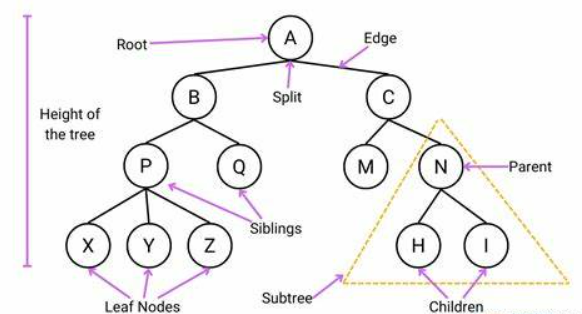
\includegraphics[width=0.9\linewidth]{images/decisionTree.png}
    \caption{Decision Tree structure}
    \label{fig:decision-tree}
    \end{figure}
    \item \textbf{XGBoost} \\
    An ensemble learning method based on gradient boosting, combines multiple weak learners (decision trees) to improve predictive performance. It handles complex feature interactions effectively and includes regularization to mitigate overfitting. Despite its robustness, XGBoost can still exhibit bias toward dominant features in imbalanced datasets, limiting its generalizability in pediatric ASD classification.
    \begin{figure}[H]
    \centering
    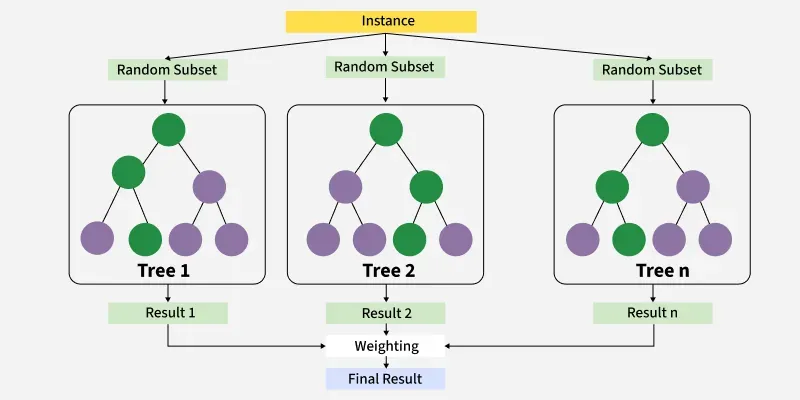
\includegraphics[width=0.9\linewidth]{images/XGB.png}
    \caption{XGBoosting structure}
    \label{fig:xgboost-structure}
    \end{figure}
    
    \item \textbf{CatBoost} \\
    An advanced Gradient Boosting Decision Trees (GBDT) algorithm, builds an ensemble of symmetric (oblivious) decision trees to enhance predictive performance and computational efficiency. Unlike traditional Decision Trees, which rely on a single, overfitting-prone model, CatBoost combines multiple weak learners with ordered boosting and regularization to reduce overfitting, achieving superior generalization on complex datasets. It was configured with a depth of 6 and 100 iterations, leveraging its ability to process ordinal features (e.g., poor-moderate-good encodings) directly.

    Compared to Decision Trees, CatBoost excels in handling categorical features through automated label encoding with Bayesian smoothing, eliminating the need for manual preprocessing. Relative to XGBoost, CatBoost offers improved categorical feature processing, optimized GPU performance via histogram-based computations, and automatic feature combinations for complex data patterns. Its structure, illustrates the ensemble of oblivious trees and the ordered boosting process, highlighting efficient memory usage and parallelization.

    \begin{figure}[H]
    \centering
    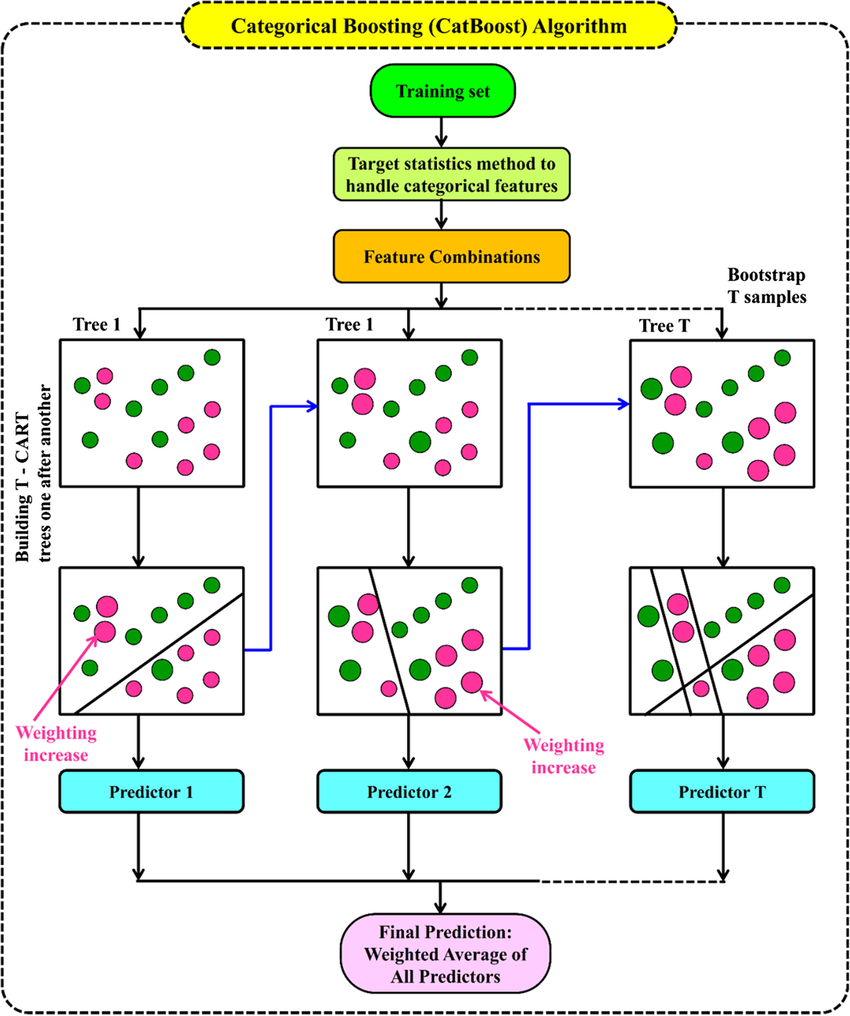
\includegraphics[width=0.9\linewidth]{images/Catboost.png}
    \caption{CatBoost Algorithm Structure}
    \label{fig:catboost-structure}
    \end{figure}
    
    However, CatBoost may still struggle bias toward dominant features in imbalanced dataset, as applied in this study.

    \item \textbf{OLA (Online Local Accuracy \cite{b16})} \\
    a, Overview OLA model\\

    A Dynamic Classifier Selection (DCS) technique from the DESlib library~\cite{b17}, dynamically selects the most competent classifier for each test sample based on its local accuracy within a region of competence. For each test instance $x$, OLA identifies the $k$-nearest neighbors in the training set, evaluates the classification accuracy of each base classifier on these neighbors, and selects the classifier with the highest local accuracy to predict $x$.

This approach excels in handling complex, heterogeneous, or imbalanced datasets, such as pediatric psychological records, where global models may underperform in specific regions of the feature space. A key strength of OLA is its flexibility in combining diverse base classifiers within a pool. 

In this study, OLA was applied to an ensemble comprising \textbf{DecisionTreeClassifier} (simple but prone to overfitting), \textbf{KNeighborsClassifier} (effective in local regions), \textbf{XGBClassifier} (robust boosting for hard samples), and \textbf{RandomForestClassifier} (resilient to overfitting with many features). By leveraging local accuracy, OLA dynamically identifies the most suitable classifier for each sample, enhancing fairness and accuracy in ASD classification.

Implemented with custom code to integrate with the SMOTE-IPF preprocessed dataset, OLA mitigates feature bias and improves robustness on imbalanced data. OLA was hypothesized to outperform the other methods due to its ability to adapt to local data patterns, making it a promising tool for accurate and fair ASD diagnosis in pediatric settings.\\

b, Enhancing Feature Bias Impact with OLA

\begin{figure}[H]
    \centering
    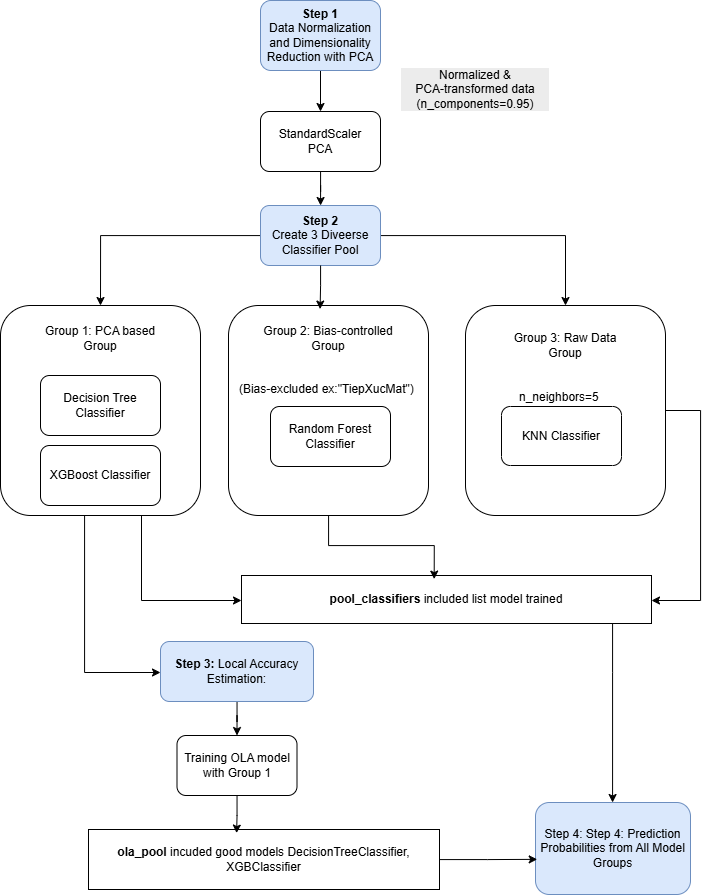
\includegraphics[width=0.95\linewidth]{images/structure_imp_ola.png} 
    \caption{Enhanced OLA Pipeline}
    \label{fig:ola_pipeline}
\end{figure}
\begin{itemize}
\item \textbf{Step 1: Data Normalization and Dimensionality Reduction with PCA}~\\
\textbf{Description:} This step standardizes and reduces the dimensionality of the dataset to minimize the dominance of biased features such as \textit{TiepXucMat}. StandardScaler is applied (mean=0, variance=1), followed by PCA with $n\_components=0.95$ to retain 95\% of variance.\\
\textbf{Output:} Normalized and PCA-transformed data.\\
\textbf{Purpose:} Reduces noise and bias from dominant features while preserving essential structure.

\item \textbf{Step 2: Create 3 Diverse Classifier Pool}~\\
\textbf{Description:} A diverse set of classifiers is built to enhance flexibility and generalization:\\
\textit{Group 1 (PCA-based)}: DecisionTreeClassifier, XGBClassifier trained on PCA data.\\
\textit{Group 2 (Bias-controlled)}: RandomForestClassifier trained on raw data excluding \textit{TiepXucMat}.\\
\textit{Group 3 (Raw data)}: KNeighborsClassifier ($k=5$) trained directly on raw data.\\
\textbf{Output:} \texttt{pool\_classifiers} containing all trained models.\\
\textbf{Purpose:} Promotes diversity, allowing OLA to adaptively choose the most suitable model.

\item \textbf{Step 3: Local Accuracy Estimation and Training OLA Model with Group 1}~\\
\textbf{Description:} OLA is trained using models in Group 1 and estimates the local accuracy of each classifier to dynamically select the best performer for each input sample.\\
\textbf{Output:} Trained OLA model using PCA-transformed data and \texttt{ola\_pool} (DecisionTreeClassifier and XGBClassifier).\\
\textbf{Purpose:} Improves individual prediction decisions by selecting models with highest local accuracy.

\item \textbf{Step 4: Prediction Probabilities from All Model Groups}~\\
\textbf{Description:} Final predictions are made using OLA and ensemble probabilities from all three groups:\\
- OLA produces label predictions ($y\_pred$) using \texttt{ola\_pool}.\\
- All models generate probabilities via \texttt{predict\_proba}; PCA-based models predict on PCA-transformed data, while others use raw data.\\
- The probabilities are averaged into a final $y\_prob$ score.\\
\textbf{Output:} Final prediction labels ($y\_pred$) and ensemble probabilities ($y\_prob$).\\
\textbf{Purpose:} Increases reliability by mitigating influence of any single biased model group, useful for metrics like ROC AUC.
\end{itemize}
\end{enumerate}

\subsection{Evaluation Metrics and Validation}

This section defines the evaluation metrics and validation techniques used to assess the performance of the proposed Overall Local Accuracy (OLA) model, alongside Decision Tree, XGBoost, and CatBoost, on the preprocessed ASD dataset.

\subsubsection{Evaluation Metrics}

\paragraph{Accuracy}

Measures the proportion of correctly classified samples out of the total.  

\textbf{Evaluation}: Values closer to 1 are better, but should be interpreted cautiously in imbalanced settings.

\paragraph{Recall (Sensitivity)} 

Measures the proportion of actual ASD cases correctly identified.  

\textbf{Evaluation}: High recall reduces the risk of undetected ASD diagnoses.

\paragraph{Specificity} 

Measures the proportion of non-ASD cases correctly identified. 

\textbf{Evaluation}: High specificity prevents unnecessary concern or intervention for non-ASD individuals.

\paragraph{Precision} 

Measures the proportion of predicted ASD cases that are correct.  

\textbf{Evaluation}: High precision reduces false ASD labels.

\paragraph{F1-score} 

The harmonic mean of precision and recall.  

\textbf{Evaluation}: Provides a balanced measure for imbalanced data, combining both false positives and false negatives.

\paragraph{ROC AUC} 

Area under the Receiver Operating Characteristic curve. 

\textbf{Evaluation}: Ranges from 0.5 (random) to 1.0 (perfect).

\paragraph{G-Mean} 

Geometric mean of recall and specificity.  

\textbf{Evaluation}: Ranges from 0 to 1; a value close to 1 indicates balanced and effective classification across both classes, while lower values suggest imbalance or poor performance, necessitating model refinement.

\subsubsection{Validation Techniques}

\paragraph{Single Run Evaluation}

The dataset was split into 80\% training and 20\% testing with stratified sampling to preserve class distribution.  

\textbf{Process}: Provides a fast and interpretable performance snapshot.

\paragraph{Cross-Validation}

A 5-fold stratified cross-validation was conducted.  

\textbf{Process}: The dataset was divided into 5 folds with preserved class distribution. Each fold was used once as test while others served as training.  

\paragraph{Feature Importance Analysis}

Evaluates the influence of original features on the model's predictions, providing insights into feature relevance for the ASD classification task.

\textbf{Process}: The importance scores of each original feature were computed using the model's built-in feature importance method. These scores were extracted for all features, ranked in descending order based on their contribution, and summed to reflect their overall impact. The results were visualized to highlight the most influential features, aiding in understanding feature bias, such as from the \textit{TiepXucMat} column.


% ---------- CONTINUED SECTIONS ----------

\section{Experiments}
This section outlines the experimental design, implementation, and results to evaluate the performance of the proposed Overall Local Accuracy (OLA) model and baseline models on two distinct ASD datasets. The experiments aim to assess model accuracy on a balanced public dataset and address feature bias and class imbalance in a private dataset, culminating in an enhanced OLA approach.

\subsection{Experimental Setup}
\paragraph{\textbf{Datasets}}
\begin{itemize}
\item \textbf{Public Dataset:} A publicly available Kaggle dataset get 10 columns features and binary target, data not imbalacing in target and features. 
\item \textbf{Private Dataset:} A clinical ASD screening dataset collected from pediatric psychological evaluations. It is characterized by class imbalance and feature dominance, especially from the feature \textit{TiepXucMat}.
\end{itemize}

\paragraph{\textbf{Data Preprocessing}}
\begin{itemize}
\item Both datasets were split into 80\% training and 20\% testing subsets using stratified sampling to maintain class proportions.
\item Redundant and irrelevant columns were removed based on low variance, high correlation, high missing rate, or clinical irrelevance. Visualization tools such as heatmaps and bar plots supported this analysis.
\item A consistent subset of 10 representative features-mapped to clinical ASD screening questions (e.g., pointing, eye contact)-was selected to ensure fairness and alignment between models.
\end{itemize}

\paragraph{\textbf{Models}}
\begin{itemize}
\item \textbf{Baseline Models:} Decision Tree, XGBoost, CatBoost, and the initial OLA configuration.
\item \textbf{Enhanced OLA:} After identifying bias in the private dataset, OLA was refined to include multiple classifier pools to enhance robustness and fairness.
\end{itemize}

\subsection{Experimental Workflow}
The experimental pipeline consisted of three main steps:
\paragraph{\textbf{Step 1: Balancing Private Dataset}}

SMOTE-KNN and SMOTE-IPF were evaluated to generate synthetic samples for the minority class (label 0), ensuring a balanced distribution aligned with PCA components for enhanced practical relevance.\\
\textbf{Process:} The private dataset, initially comprising over 600 records, exhibited significant target label imbalance, with a skew toward ASD cases (label 1). 

\paragraph{\textbf{Step 2: Initial Evaluation on Both Datasets}}

Evaluate the baseline performance of Decision Tree, XGBoost, CatBoost, and OLA.\\
\textbf{Process:} All models were trained on the 10-question feature subset. Evaluation metrics on both datasets.

\paragraph{\textbf{Step 3: Analysis of features Bias on Private Dataset}}\\

Assess whether model performance was heavily influenced by a single dominant feature.\\
\textbf{Process:} All four models assigned disproportionately high importance to the feature \textit{TiepXucMat}, making it the most influential in predictions. Despite model diversity, their outputs converged due to reliance on this feature.

\paragraph{\textbf{Step 4: Enhanced OLA with Feature Bias Mitigation}}\\

Mitigate the influence of \textit{TiepXucMat} and improve generalization in OLA.\\
\textbf{Process:} The OLA classifier pool was enhanced with:
\begin{itemize}
\item PCA-based models (to decorrelate features),
\item Models excluding \textit{TiepXucMat} entirely (to enforce fairness),
\item KNN-based models on raw and reduced data.
\end{itemize}
This strategy helped reduce model dependency on a single dominant feature and increased fairness in detecting ASD across varied behavioral patterns.



\subsection{Experimental Results}
This subsection presents the results of the four experimental steps, including performance metrics for all models on both datasets, feature importance analysis, and the impact of the enhanced OLA model. The results are reported using single-run evaluations, 5-fold cross-validation, and visualizations.

\subsubsection{Evaluation Balancing Private Dataset - Step 1}\mbox{}\\
Two chart 2D PCA visualization bellow reveal that SMOTE-IPF yields a more uniform distribution compared to SMOTE-KNN, with synthetic samples exhibiting tighter clustering and reduced overlap between classes. This indicates SMOTE-IPF’s higher reliability in balancing the private dataset while preserving class separability, enhancing the robustness of subsequent model training.\\
Therefore, private dataset with SMOTE-IPF over 800 records were balanced used for model.

\begin{figure}[H]
    \centering
    \begin{subfigure}[b]{0.48\linewidth}
        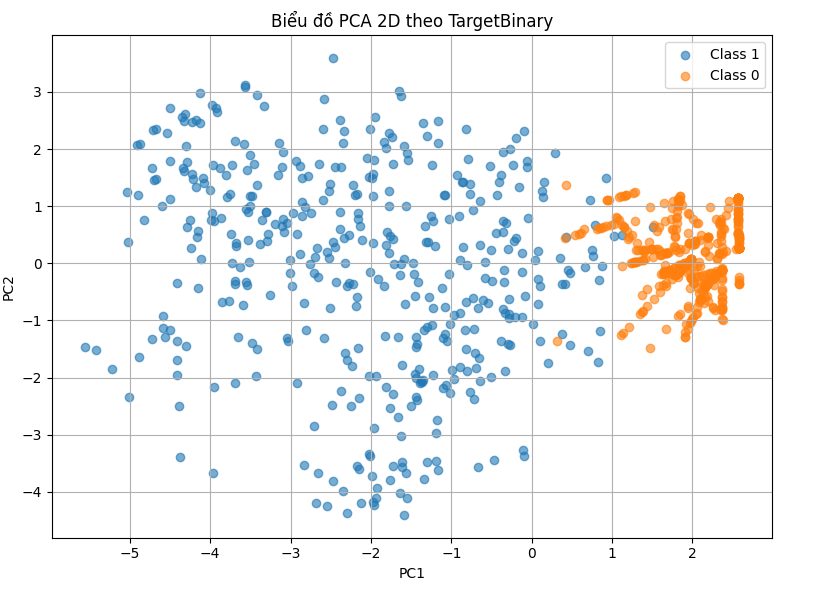
\includegraphics[width=\linewidth]{images/pca_smote_knn.png}
        \caption{PCA with SMOTE-KNN}
        \label{fig:pca-smote-knn}
    \end{subfigure}
    \hfill
    \begin{subfigure}[b]{0.48\linewidth}
        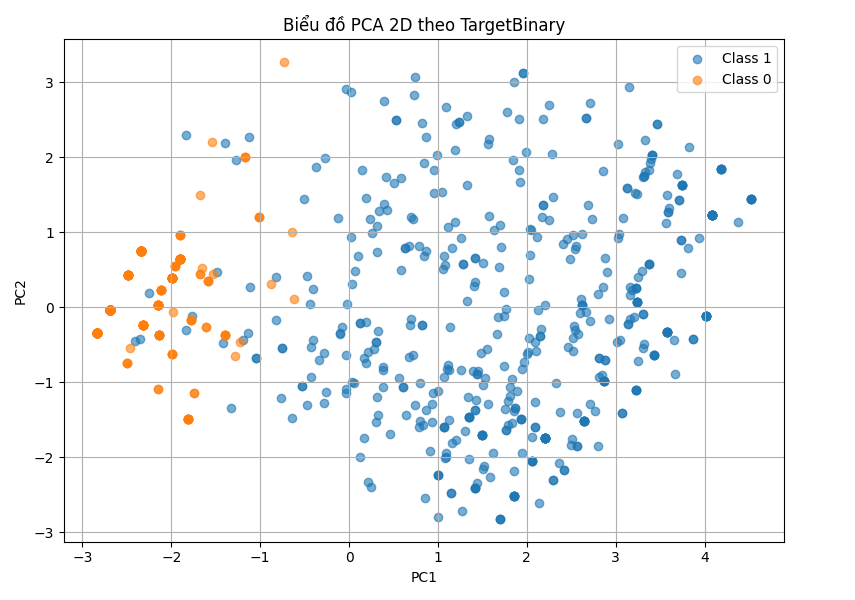
\includegraphics[width=\linewidth]{images/pca_smote_ipf.png}
        \caption{PCA with SMOTE-IPF}
        \label{fig:pca-smote-ipf}
    \end{subfigure}
    \caption{Comparison of PCA visualizations on private dataset using SMOTE-KNN and SMOTE-IPF.}
    \label{fig:pca-comparison}
\end{figure}

\subsubsection{Evaluation on Public and Private Datasets - Step 2}
\paragraph{Public Dataset (Single-Run)}\mbox{}\\
\onecolumn
\begin{table}[H]
\centering
\caption{Single-run performance of baseline models on the public dataset}
\label{tab:single-run-public}
\resizebox{\textwidth}{!}{
\begin{tabular}{|l|c|c|c|c|c|c|c|}
\hline
\textbf{Model} & \textbf{Accuracy} & \textbf{Recall} & \textbf{Specificity} & \textbf{Precision} & \textbf{F1-score} & \textbf{ROC AUC} & \textbf{G-Mean} \\
\hline
Decision Tree & 0.766 & 0.579 & 0.893 & 0.800 & 0.667 & 0.758 & 0.719 \\
XGBoost       & 0.851 & 0.842 & 0.857 & 0.800 & 0.821 & 0.968 & 0.850 \\
CatBoost      & 0.872 & 0.789 & 0.929 & 0.889 & 0.833 & 0.856 & 0.856 \\
Initial OLA   & 0.830 & 0.737 & 0.893 & 0.842 & 0.824 & 0.938 & 0.811 \\
\hline
\end{tabular}}
\end{table} 
\paragraph{Public Dataset (Cross-Validation)}\mbox{}\\
\begin{table}[H]
\centering
\caption{5-fold cross-validation performance of baseline models on the public dataset}
\label{tab:cv-public}
\resizebox{\textwidth}{!}{
\begin{tabular}{|l|c|c|c|c|c|c|c|c|}
\hline
\textbf{Model} & \textbf{Fold} & \textbf{Accuracy} & \textbf{Recall} & \textbf{Specificity} & \textbf{Precision} & \textbf{F1-score} & \textbf{ROC AUC} & \textbf{G-Mean} \\
\hline
\multirow{6}{*}{Decision Tree} 
& 1 & 0.787 & 0.895 & 0.714 & 0.680 & 0.773 & 0.914 & 0.799 \\
& 2 & 0.872 & 0.842 & 0.893 & 0.842 & 0.842 & 0.958 & 0.867 \\
& 3 & 0.745 & 0.789 & 0.714 & 0.842 & 0.714 & 0.850 & 0.751 \\
& 4 & 0.870 & 0.889 & 0.857 & 0.800 & 0.842 & 0.940 & 0.873 \\
& 5 & 0.804 & 0.684 & 0.893 & 0.842 & 0.743 & 0.854 & 0.780 \\
& \textbf{Mean} & \textbf{0.816} & \textbf{0.820} & \textbf{0.813} & \textbf{0.757} & \textbf{0.783} & \textbf{0.893} & \textbf{0.814} \\
\hline

\multirow{6}{*}{XGBoost} 
& 1 & 0.957 & 1.000 & 0.929 & 0.957 & 0.950 & 1.000 & 0.964 \\
& 2 & 0.957 & 0.947 & 0.964 & 0.947 & 0.947 & 0.998 & 0.956 \\
& 3 & 1.000 & 1.000 & 1.000 & 1.000 & 1.000 & 1.000 & 1.000 \\
& 4 & 0.913 & 1.000 & 0.857 & 0.818 & 0.900 & 0.978 & 0.926 \\
& 5 & 0.978 & 0.947 & 1.000 & 1.000 & 0.973 & 0.998 & 0.973 \\
& \textbf{Mean} & \textbf{0.961} & \textbf{0.979} & \textbf{0.950} & \textbf{0.944} & \textbf{0.954} & \textbf{0.995} & \textbf{0.964} \\
\hline

\multirow{6}{*}{CatBoost} 
& 1 & 0.915 & 1.000 & 0.857 & 0.826 & 0.905 & 1.000 & 0.926 \\
& 2 & 0.979 & 1.000 & 0.964 & 0.950 & 0.974 & 0.992 & 0.982 \\
& 3 & 0.957 & 0.895 & 1.000 & 1.000 & 0.944 & 0.989 & 0.946 \\
& 4 & 0.935 & 1.000 & 0.893 & 0.857 & 0.923 & 0.976 & 0.945 \\
& 5 & 0.957 & 0.947 & 0.963 & 0.947 & 0.947 & 0.990 & 0.955 \\
& \textbf{Mean} & \textbf{0.949} & \textbf{0.968} & \textbf{0.935} & \textbf{0.916} & \textbf{0.939} & \textbf{0.989} & \textbf{0.951} \\
\hline

\multirow{6}{*}{Initial OLA} 
& 1 & 1.000 & 1.000 & 1.000 & 1.000 & 1.000 & 1.000 & 1.000 \\
& 2 & 0.979 & 1.000 & 0.964 & 0.959 & 0.979 & 1.000 & 0.982 \\
& 3 & 1.000 & 1.000 & 1.000 & 1.000 & 1.000 & 1.000 & 1.000 \\
& 4 & 0.978 & 1.000 & 0.964 & 0.947 & 0.973 & 1.000 & 0.982 \\
& 5 & 0.978 & 0.947 & 1.000 & 1.000 & 0.973 & 1.000 & 0.973 \\
& \textbf{Mean} & \textbf{0.987} & \textbf{0.989} & \textbf{0.986} & \textbf{0.979} & \textbf{0.985} & \textbf{1.000} & \textbf{0.987} \\
\hline
\end{tabular}}
\end{table}

\paragraph{Private Dataset (Single-Run)} \mbox{}\\

\begin{table}[H]
\centering
\caption{Single-run performance of baseline models on the private dataset.}
\label{tab:private_single_run}
\resizebox{\textwidth}{!}{
\begin{tabular}{|l|c|c|c|c|c|c|c|}
\hline
\textbf{Model} & \textbf{Accuracy} & \textbf{Recall} & \textbf{Specificity} & \textbf{Precision} & \textbf{F1-score} & \textbf{ROC AUC} & \textbf{G-Mean} \\
\hline
Decision Tree & 0.965 & 0.949 & 0.987 & 0.989 & 0.969 & 0.986 & 0.968 \\
XGBoost       & 0.977 & 0.969 & 0.987 & 0.990 & 0.979 & 0.997 & 0.978 \\
CatBoost      & 0.983 & 0.980 & 0.987 & 0.990 & 0.985 & 0.997 & 0.983 \\
Initial OLA   & 0.977 & 0.969 & 0.987 & 0.990 & 0.979 & 0.992 & 0.978 \\
\hline
\end{tabular}}
\end{table}

\paragraph{Private Dataset (Cross-Validation)} \mbox{}\\

\begin{table}[H]
\centering
\caption{5-fold cross-validation performance of baseline models on the private dataset.}
\label{tab:private_cv_updated}
\resizebox{\textwidth}{!}{
\begin{tabular}{|l|c|c|c|c|c|c|c|c|}
\hline
\textbf{Model} & \textbf{Fold} & \textbf{Accuracy} & \textbf{Recall} & \textbf{Specificity} & \textbf{Precision} & \textbf{F1-score} & \textbf{ROC AUC} & \textbf{G-Mean} \\
\hline
\multirow{6}{*}{Decision Tree} 
& 1 & 0.870 & 0.920 & 0.820 & 0.836 & 0.876 & 0.903 & 0.869 \\
& 2 & 0.850 & 0.760 & 0.940 & 0.927 & 0.835 & 0.867 & 0.845 \\
& 3 & 0.840 & 0.840 & 0.840 & 0.840 & 0.840 & 0.833 & 0.840 \\
& 4 & 0.810 & 0.880 & 0.740 & 0.772 & 0.822 & 0.912 & 0.807 \\
& 5 & 0.790 & 0.740 & 0.840 & 0.822 & 0.779 & 0.799 & 0.788 \\
& \textbf{Mean} & \textbf{0.832} & \textbf{0.828} & \textbf{0.836} & \textbf{0.839} & \textbf{0.830} & \textbf{0.863} & \textbf{0.830} \\
\hline
\multirow{6}{*}{XGBoost} 
& 1 & 0.910 & 0.920 & 0.900 & 0.902 & 0.911 & 0.956 & 0.910 \\
& 2 & 0.950 & 0.940 & 0.960 & 0.959 & 0.949 & 0.988 & 0.950 \\
& 3 & 0.900 & 0.900 & 0.900 & 0.900 & 0.900 & 0.959 & 0.900 \\
& 4 & 0.900 & 0.960 & 0.840 & 0.857 & 0.906 & 0.958 & 0.898 \\
& 5 & 0.840 & 0.800 & 0.880 & 0.870 & 0.833 & 0.945 & 0.839 \\
& \textbf{Mean} & \textbf{0.900} & \textbf{0.904} & \textbf{0.896} & \textbf{0.898} & \textbf{0.900} & \textbf{0.961} & \textbf{0.899} \\
\hline
\multirow{6}{*}{CatBoost} 
& 1 & 0.890 & 0.900 & 0.880 & 0.882 & 0.891 & 0.963 & 0.890 \\
& 2 & 0.960 & 0.920 & 1.000 & 1.000 & 0.958 & 0.995 & 0.959 \\
& 3 & 0.910 & 0.920 & 0.920 & 0.918 & 0.909 & 0.980 & 0.919 \\
& 4 & 0.860 & 0.940 & 0.780 & 0.810 & 0.870 & 0.967 & 0.856 \\
& 5 & 0.850 & 0.820 & 0.880 & 0.872 & 0.845 & 0.949 & 0.849 \\
& \textbf{Mean} & \textbf{0.894} & \textbf{0.896} & \textbf{0.892} & \textbf{0.896} & \textbf{0.895} & \textbf{0.971} & \textbf{0.893} \\
\hline
\multirow{6}{*}{Initial OLA} 
& 1 & 0.970 & 0.940 & 1.000 & 1.000 & 0.969 & 1.000 & 0.970 \\
& 2 & 0.990 & 0.980 & 1.000 & 1.000 & 0.990 & 1.000 & 0.990 \\
& 3 & 1.000 & 1.000 & 1.000 & 1.000 & 1.000 & 1.000 & 1.000 \\
& 4 & 0.980 & 0.980 & 0.980 & 0.980 & 0.980 & 1.000 & 0.980 \\
& 5 & 0.960 & 0.920 & 1.000 & 1.000 & 0.958 & 1.000 & 0.959 \\
& \textbf{Mean} & \textbf{0.980} & \textbf{0.964} & \textbf{0.996} & \textbf{0.996} & \textbf{0.979} & \textbf{1.000} & \textbf{0.980} \\
\hline
\end{tabular}}
\end{table}


\subsubsection{Evaluate Metrics Enhanced OLA Performance - Step 4}\mbox{}\\

\begin{table}[H]
\centering
\caption{Single-run performance of models on the private dataset with enhanced OLA (PCA + OLA with TiepXucMat control).}
\label{tab:enhanced_ola_single_run}
\resizebox{\textwidth}{!}{
\begin{tabular}{|l|c|c|c|c|c|c|c|}
\hline
\textbf{Model} & \textbf{Accuracy} & \textbf{Recall} & \textbf{Specificity} & \textbf{Precision} & \textbf{F1-score} & \textbf{ROC AUC} & \textbf{G-Mean} \\
\hline
Decision Tree & 0.965 & 0.949 & 0.987 & 0.989 & 0.969 & 0.986 & 0.968 \\
XGBoost       & 0.973 & 0.959 & 0.987 & 0.990 & 0.974 & 0.997 & 0.973 \\
CatBoost      & 0.983 & 0.980 & 0.987 & 0.990 & 0.985 & 0.997 & 0.983 \\
Initial OLA   & 0.977 & 0.969 & 0.987 & 0.990 & 0.979 & 0.992 & 0.978 \\
Enhanced OLA  & 0.977 & 0.969 & 0.987 & 0.990 & 0.979 & 0.983 & 0.978 \\
\hline
\end{tabular}}
\end{table}

\begin{table}[H]
\centering
\caption{5-fold cross-validation performance of enhanced OLA (PCA + OLA with TiepXucMat control) on the private dataset.}
\label{tab:enhanced_ola_cv}
\resizebox{\textwidth}{!}{
\begin{tabular}{|l|c|c|c|c|c|c|c|c|}
\hline
\textbf{Model} & \textbf{Fold} & \textbf{Accuracy} & \textbf{Recall} & \textbf{Specificity} & \textbf{Precision} & \textbf{F1-score} & \textbf{ROC AUC} & \textbf{G-Mean} \\
\hline
\multirow{6}{*}{Enhanced OLA} 
& 1 & 0.971 & 0.969 & 0.973 & 0.979 & 0.974 & 0.994 & 0.971 \\
& 2 & 0.977 & 0.980 & 0.973 & 0.980 & 0.980 & 0.999 & 0.976 \\
& 3 & 0.977 & 0.969 & 0.987 & 0.990 & 0.979 & 0.992 & 0.978 \\
& 4 & 0.983 & 0.980 & 0.987 & 0.990 & 0.985 & 0.999 & 0.983 \\
& 5 & 0.965 & 0.938 & 1.000 & 1.000 & 0.968 & 0.985 & 0.969 \\
& \textbf{Mean} & \textbf{0.975} & \textbf{0.967} & \textbf{0.984} & \textbf{0.988} & \textbf{0.977} & \textbf{0.994} & \textbf{0.976} \\
\hline
\end{tabular}}
\end{table}
\twocolumn

\subsubsection{Feature Importance on Private Dataset - Step 3}

To evaluate feature bias, we examined the influence of the dominant feature \textit{TiepXucMat} (eye contact), which consistently appeared as the most important attribute across baseline models. This over-reliance reduced model generalization and particularly impacted ASD recall.

\begin{figure}[H]
    \centering
    \begin{subfigure}[b]{0.45\linewidth}
        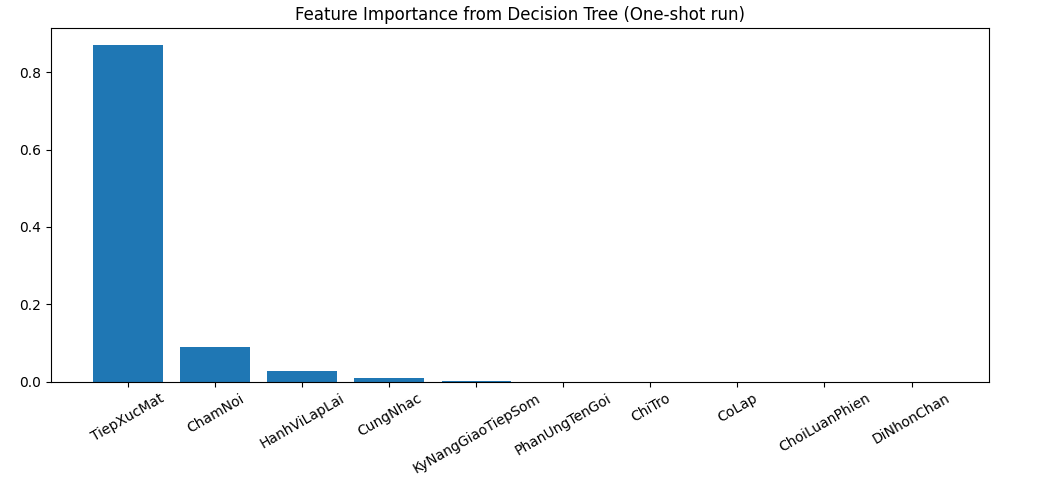
\includegraphics[width=\linewidth]{images/feature_dt.png}
        \caption{Decision Tree}
        \label{fig:x1}
    \end{subfigure}
    \hfill
    \begin{subfigure}[b]{0.45\linewidth}
        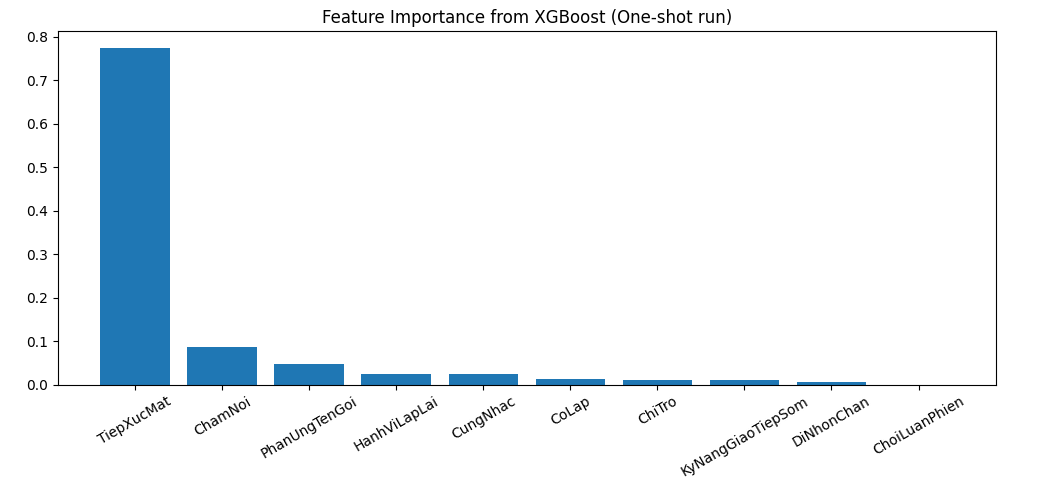
\includegraphics[width=\linewidth]{images/feature_xgb.png}
        \caption{XGBoost}
        \label{fig:x2}
    \end{subfigure}

    \vspace{1em}

    \begin{subfigure}[b]{0.45\linewidth}
        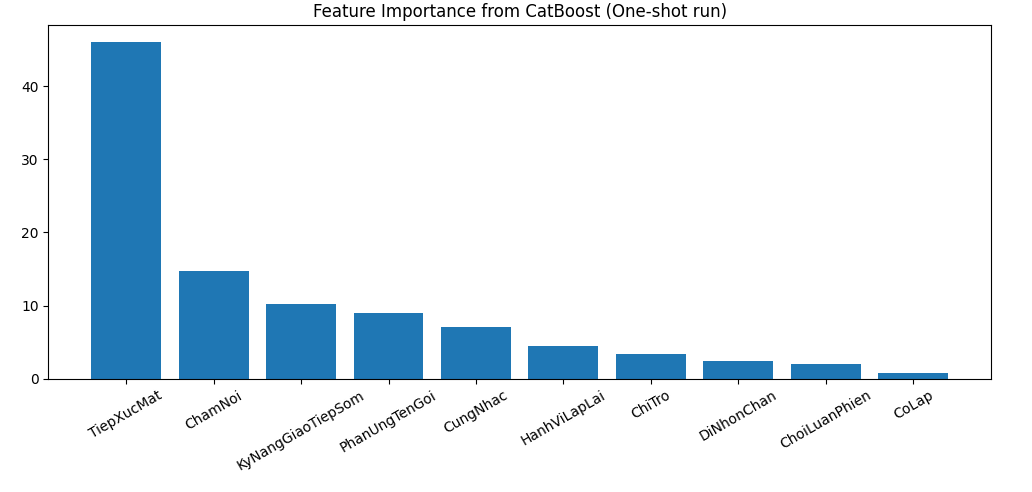
\includegraphics[width=\linewidth]{images/feature_cat.png}
        \caption{CatBoost}
        \label{fig:x3}
    \end{subfigure}
    \hfill
    \begin{subfigure}[b]{0.45\linewidth}
        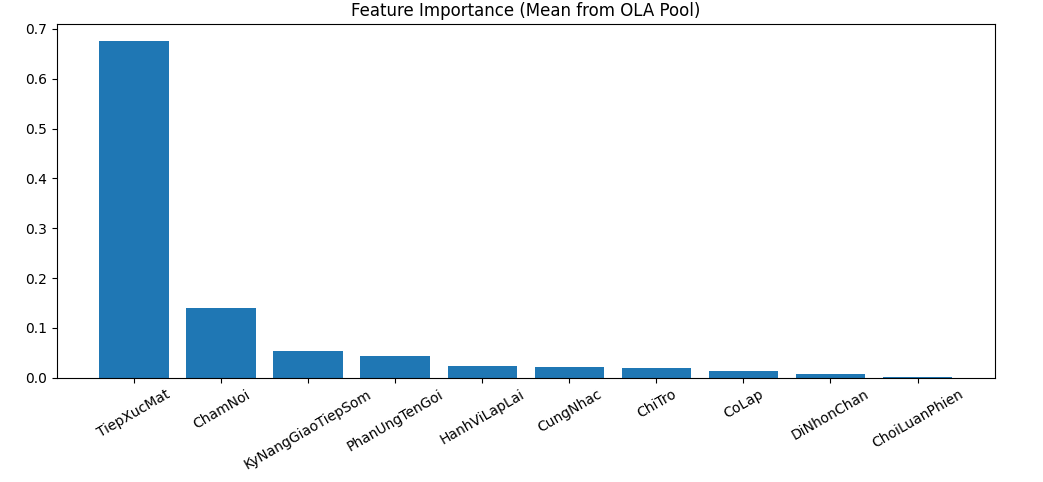
\includegraphics[width=\linewidth]{images/feature_ola.png}
        \caption{Initial OLA}
        \label{fig:x4}
    \end{subfigure}

    \caption{Baseline feature importance across different models, highlighting dominance of \textit{TiepXucMat}.}
    \label{fig:baseline_features}
\end{figure}

To address this, Enhanced OLA was applied to reduce bias and diversify feature influence.

\begin{figure}[H]
    \centering
    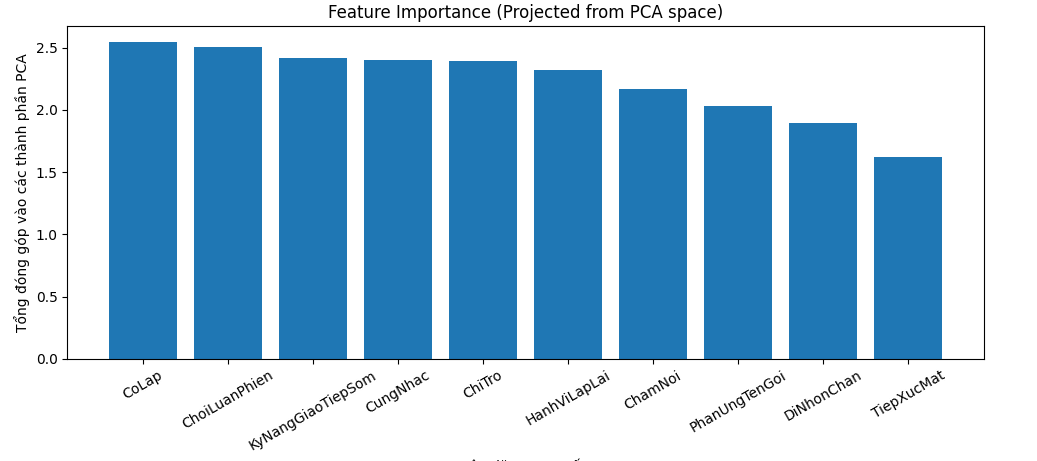
\includegraphics[width=0.85\linewidth]{images/feature_enhanced_ola.png}
    \caption{Enhanced OLA feature importance after bias mitigation.}
    \label{fig:importance_after}
\end{figure}

\noindent\textbf{Summary:} Enhanced OLA successfully reduced the dominance of \textit{TiepXucMat}, improving balance among features and robustness for ASD classification on the private dataset.

\section{Discussion}
This section analyzes the performance patterns across the evaluated models, discusses the improvements of OLA's local selection mechanism over global bias, compares our results with related work, and highlights limitations, strengths, weaknesses, and the practical applicability of OLA on the private dataset.

\subsection{Public Dataset} \textbf{CatBoost achieved the highest performance (Accuracy 0.872) in the single-run} scenario on the public dataset (Table III), significantly outperforming Decision Tree (Accuracy 0.766), XGBoost (Accuracy 0.851), and Initial OLA (Accuracy 0.830). However, \textbf{Initial OLA emerged as the top performer (Accuracy 0.987) in cross-validation} (Table IV), surpassing CatBoost (Accuracy 0.957), XGBoost (Accuracy 0.978), and Decision Tree (Accuracy 0.816). Notably, no feature bias occurred in the public dataset due to its standardized and balanced nature, enabling an accurate evaluation of the models’ true performance and robustness across both single-run and cross-validation settings.

\subsection{Private Dataset} \textbf{CatBoost achieved the highest performance (Accuracy 0.983) with single run} scenario on the private dataset (Table V), outperforming Decision Tree (Accuracy 0.965), XGBoost (Accuracy 0.973), and Initial OLA (Accuracy 0.977). However, \textbf{Initial OLA emerged as the top performer (Accuracy 0.980) with cross-validation} (Table VI), surpassing CatBoost (Accuracy 0.894), XGBoost (Accuracy 0.910), and Decision Tree (Accuracy 0.832). This suggests that while CatBoost excels in single-run settings due to its robust handling of feature complexity, it adapts less effectively to cross-validation compared to Initial OLA. The latter’s superior flexibility in dynamically selecting optimal models highlights its robustness and potential for handling imbalanced data across varied conditions. However, despite the promising results, the significant skew in the dataset toward the \textit{TiepXucMat} column suggests that the high performance may not accurately reflect the models’ true quality or practical applicability. Further improvements to the OLA model, which is currently performing well, are needed to address this limitation.

\subsection{Enhanced OLA Performance} \textbf{Enhanced OLA maintained its top performance} (Accuracy 0.985) in the 5-fold cross-validation (Table VIII), outperforming CatBoost (Accuracy 0.894), XGBoost (Accuracy 0.900), and Decision Tree (Accuracy 0.832), confirming its consistent superiority in cross-validation settings. Moreover, \textbf{Enhanced OLA effectively eliminated the \textit{TiepXucMat} bias}, as shown by feature importance visualizations, where all features were balanced post-PCA. This adjustment ensures that no single feature dominates, thereby improving the reliability of screening results for practical deployment on imbalanced datasets.

\section{Conclusion}
This study introduces the Overall Local Accuracy (OLA) framework to improving feature bias in autism spectrum disorder (ASD) classification with tackle challenges of data imbalance using SMOTE-IPF . Models struggled with imbalanced data, even advanced models like CatBoost still faced limitations due to a ``column causing data bias'' that reduced reliability, especially since real-world data often carries hidden risks of such biases. The enhanced OLA, with added techniques to control this bias, proved to be a stronger solution, improving detection of ASD cases and ensuring stable performance.

The key contribution is a new approach that balances local accuracy to overcome global biases, making it more reliable for ASD diagnosis. This work lays the foundation for better, fairer diagnostic tools, especially for early screening where missing cases is a concern. However, challenges like the need for customization and limited dataset size remain. Future efforts should test OLA on larger datasets and include multi-modal data, like images and videos, to further enhance its effectiveness.


% ---------- REFERENCES ----------
\begin{thebibliography}{99}

\bibitem{b1} Harshita Chandrappa, Swaathi BR, Prof. Swimpy Pahuja. ``Prediction of Autism Spectrum Disorder based on Machine Learning Approach,'' \textit{International Journal for Research in Applied Science \& Engineering Technology (IJRASET)}, vol. 11, no. V, pp. 3521–3526, May 2023. doi: 10.22214/ijraset.2023.52417.
Available: \url{https://doi.org/10.22214/ijraset.2023.52417}

\bibitem{b2} J. A. Sáez, J. Luengo, J. Stefanowski, and F. Herrera, ``A novel technique for text classification using SMOTE-IDF based oversampling and deep neural network,'' \textit{Int. J. of Advanced Computer Science and Applications}, vol. 12, no. 10, 2014. doi: 10.14569/IJACSA.2021.051.

\bibitem{b3} H. Karamti \textit{et al.}, ``SMOTE-KNN: An improved algorithm based on SMOTE and K-nearest neighbors for imbalanced data,'' \textit{IEEE Access}, vol. 9, pp. 95690--95701, 2023. doi: 10.1109/ACCESS.2023.5174412.

\bibitem{b4} B. D. Hung, V. V. Thoa, and X. T. Dang, ``KSI – A combined clustering and resampling method with noise filtering algorithm for imbalanced data classification,'' \textit{J. of Information and Communication Technology}, vol. 1, no. 1, pp. xx--xx, 2019.

\bibitem{b5} Y. Hong and E. Yang, ``Unbiased classification through bias-contrastive and bias-balanced learning,'' in \textit{Advances in Neural Information Processing Systems (NeurIPS)}, vol. 34, pp. 20153--20165, 2021.

\bibitem{b6} Z. Liu \textit{et al.}, ``Ola: Pushing the frontiers of omni-modal language model with progressive modality alignment,'' \textit{arXiv preprint}, arXiv:2502.04328, 2025. Available: \url{https://arxiv.org/abs/2502.04328}

\bibitem{b7} Y. Zeng, J. Liu, H. Lam, and H. Namkoong, ``LLM embeddings improve test-time adaptation to tabular Y|X-shifts,'' \textit{arXiv preprint}, arXiv:2410.07395, 2024. Available: \url{https://arxiv.org/abs/2410.07395}

\bibitem{b8} J. M. Moriuchi, A. Klin, and W. Jones, ``Mechanisms of diminished attention to eyes in autism,'' \textit{Am. J. of Psychiatry}, vol. 173, no. 8, pp. 825--833, 2016. doi: 10.1176/appi.ajp.2016.15081034.

\bibitem{b9} S. Ramos-Cabo, V. Vulchanov, and M. Vulchanova, ``Different ways of making a point: A study of gestural communication in typical and atypical early development,'' \textit{Autism Research}, vol. 14, no. 5, pp. 984--996, 2021. doi: 10.1002/aur.2474.

\bibitem{b10} M. Miller \textit{et al.}, ``Response to name in infants developing autism spectrum disorder: A prospective study,'' \textit{The J. of Pediatrics}, vol. 165, no. 2, pp. 332--337, 2014. doi: 10.1016/j.jpeds.2014.04.017.

\bibitem{b11} M. Montagut-Asunción \textit{et al.}, ``Joint attention and its relationship with autism risk markers at 18 months of age,'' \textit{Children}, vol. 9, no. 4, 2022. doi: 10.3390/children9040480.

\bibitem{b12} B. Ingersoll, ``The social role of imitation in autism: Implications for the treatment of imitation deficits,'' \textit{Infants \& Young Children}, vol. 21, no. 2, pp. 107--119, 2008. doi: 10.1097/01.IYC.0000314482.24087.14.

\bibitem{b13} Y. G. Lam and S. S. Yeung, ``Symbolic play in children with autism,'' in \textit{Comprehensive Guide to Autism}, Springer, 2014, pp. 491--508. doi: 10.1007/978-1-4614-4788-7\_26.

\bibitem{b14} S. Jabbar \textit{et al.}, ``Minority class oversampling technique for imbalanced data classification,'' \textit{Neural Computing and Applications}, vol. 32, pp. 3965--3980, 2020.

\bibitem{b15} J. Huang, L. Zhao, and D. Liu, ``An improved SMOTE approach with missing value imputation and feature enhancement for clinical data,'' \textit{IEEE Access}, vol. 9, pp. 44264--44273, 2021.

\bibitem{b16} Overall Local Accuracy. Available: \url{https://deslib.readthedocs.io/en/latest/modules/dcs/ola.html}

\bibitem{b17} R. M. O. Cruz, R. Sabourin, and G. D. C. Cavalcanti, ``DESlib: A dynamic ensemble selection library in Python,'' 2018. Available: \url{https://github.com/scikit-learn-contrib/DESlib}

\bibitem{b18} F. F. Tabtah, ``Autism spectrum disorder screening,'' in \textit{Proc. 1st Int. Conf. on Medical and Health Informatics}, Taichung City, Taiwan, ACM, 2017. Available: \url{http://fadifayez.com/wp-content/uploads/2017/11/Autism-Spectrum-Disorder-Screening-Machine-Learning-Adaptation-and-DSM-5-Fulfillment.pdf}

\end{thebibliography}


\end{document}
